\chapter{BVRP previsto e retornos futuros: modelo linear}
\label{chap:retornos_linear}

Este capítulo testa se o BVRP previsto no Capítulo~\ref{chap:previsao_bvrp}
prevê linearmente os retornos futuros do Bitcoin. O coeficiente é negativo em
todos os seis horizontes e nos dois modelos de previsão: um BVRP previsto mais
alto, isto é, um prêmio de variância menor, antecede retornos menores. Nenhum
horizonte, porém, é significante depois de duas correções necessárias: a da
incerteza do BVRP previsto, que é um regressor gerado, e a das comparações
múltiplas. O teste conjunto nos seis horizontes só rejeita quando ignora a
estimação do BVRP previsto.

% =========================================================
\section{Especificação}
\label{sec:retlin-especificacao}

Para cada horizonte $h \in \{1, 5, 10, 20, 30, 60\}$ dias, a dissertação
estima a equação~\eqref{eq:met-retorno-linear},
\[
R_{t+h} = \alpha_h + \beta_h \, \widehat{\text{BVRP}}_t + \varepsilon_{t+h},
\]
por MQO, nas 987 datas fora da amostra do Capítulo~\ref{chap:previsao_bvrp}
(21/06/2023 a 03/03/2026). $R_{t+h}$ é o retorno simples de $t$ a $t+h$, e
$\widehat{\text{BVRP}}_t$, a previsão do Ridge na janela expansiva. A previsão
da floresta aleatória serve de teste de robustez; as duas escolhas foram
fixadas antes de ver os resultados deste capítulo
(Seção~\ref{sec:prev-sintese}). Os coeficientes são reportados em pontos
percentuais de retorno por ponto percentual de BVRP previsto.

A especificação é preditiva: $\beta_h$ mede se o BVRP previsto em $t$
antecipa o retorno dos $h$ dias seguintes, e não o efeito causal do prêmio
sobre o preço. Os retornos de datas vizinhas se sobrepõem em $h-1$ dias, o que
induz autocorrelação nos erros. A correção para essa sobreposição é feita no
erro-padrão, e não no estimador: o $\hat\beta_h$ é o mesmo do MQO, e o
erro-padrão de Newey--West com $h+1$ defasagens contorna a autocorrelação sob
as condições da Seção~\ref{sec:met-inferencia}. Mesmo com essa correção,
regressões com retornos sobrepostos podem sofrer distorções em amostras
finitas, que \citet{bollerslev2014international} avaliam por simulação, e os
testes têm pouco poder nos horizontes longos: em $h = 60$, as 987 datas contêm só cerca de 16
períodos sem sobreposição.

% =========================================================
\section{Inferência com o BVRP previsto}
\label{sec:retlin-inferencia}

O erro-padrão HAC trata $\widehat{\text{BVRP}}_t$ como se fosse observado,
quando ele é estimado no primeiro estágio \citep{pagan1984}. Por isso, a
inferência principal usa o bootstrap em blocos em dois níveis da
Seção~\ref{sec:met-inferencia} \citep{kunsch1989}, um procedimento não
paramétrico: em cada reamostragem, o modelo de previsão é reestimado em cada
origem, com um treino reamostrado em blocos dentro da própria janela de
treino, e $\beta_h$ é reestimado com os pares (previsão, retorno) das 987
datas, também reamostrados em blocos.\footnote{No principal, o $\alpha$ do
Ridge fica fixo, em cada origem, no valor escolhido no
Capítulo~\ref{chap:previsao_bvrp}. Reescolhê-lo por validação cruzada em
cada treino reamostrado distorce o procedimento: blocos repetidos podem cair
no treino e na validação da mesma dobra, e a validação passa a favorecer
penalidades menores. O resultado com o $\alpha$ reescolhido aparece entre os
testes de robustez (Seção~\ref{sec:retlin-robustez}).} A reestimação do
primeiro estágio acrescenta ruído à previsão e, como em todo problema de erro
nas variáveis, atenua o coeficiente: a média dos $\beta^*$ das reamostragens
fica abaixo de $\hat\beta_h$, em módulo. A razão $\lambda_h$ entre as duas
mede essa atenuação e fica entre 0,59 e 0,70. O $\hat\beta_h$ estimado com o
BVRP previsto é, portanto, uma medida conservadora da relação entre o prêmio
e o retorno futuro.

A atenuação também encolhe a dispersão dos $\beta^*$, e comparar
$\hat\beta_h$, que não é atenuado, com o erro-padrão do bootstrap, que é,
misturaria escalas e daria valores-$p$ pequenos demais. O teste usa, por
isso, a mesma escala nos dois termos: o erro-padrão de $\hat\beta_h$ é o do
bootstrap dividido por $\lambda_h$, e o intervalo de confiança é
$\hat\beta_h \pm 1{,}96$ vezes esse erro-padrão.\footnote{Com blocos de 60
dias, o segundo nível reamostra cerca de 16 blocos, e intervalos por
percentis seriam grosseiros; por isso o intervalo usa o erro-padrão. Nas
junções entre blocos, a ordem temporal deixa de valer, limitação comum aos
bootstraps em blocos.} O erro-padrão corrigido fica entre 1,25 e 1,71 vez o
HAC. Com seis horizontes, o limite de Bonferroni é
$0{,}05/6 \approx 0{,}0083$.

% =========================================================
\section{Resultados}
\label{sec:retlin-resultados}

A Tabela~\ref{tab:retlin-principal} e a Figura~\ref{fig:retlin-betas}
apresentam os resultados. O coeficiente é negativo em todos os horizontes e
cresce em módulo com $h$, de $-0{,}045$ em $h = 1$ a $-1{,}43$ em $h = 60$.
Em $h = 30$, um desvio-padrão da previsão do Ridge (4,5 p.p.) corresponde a
cerca de 2,6 p.p. a menos de retorno em 30 dias. Com o erro-padrão HAC, os
valores-$p$ ficam entre 0,011 e 0,091; com o bootstrap em dois níveis, entre
0,043 ($h = 1$) e 0,30. Só $h = 1$ fica abaixo de 0,05 no bootstrap, e nenhum
horizonte passa pelo limite de Bonferroni, nem com o HAC.

\begin{table}[H]
\centering
\footnotesize
\caption{Retorno futuro sobre o BVRP previsto: estimativas e inferência por horizonte.}
\label{tab:retlin-principal}
\begin{tabular}{rrrrrrrcr}
\toprule
 & & \multicolumn{2}{c}{HAC} & \multicolumn{4}{c}{Bootstrap em dois níveis} & \\ \cmidrule(lr){3-4}\cmidrule(lr){5-8}
$h$ & $\hat\beta_h$ & EP & $p$ & $\lambda$ & EP corrigido & $p$ & IC 95\% & $R^2$ \\
\midrule
1 & $-$0{,}045 & 0{,}018 & 0{,}011 & 0{,}59 & 0{,}022 & 0{,}043 & [$-$0{,}089; $-$0{,}001] & 0{,}007 \\
5 & $-$0{,}144 & 0{,}064 & 0{,}025 & 0{,}68 & 0{,}082 & 0{,}080 & [$-$0{,}306; 0{,}017] & 0{,}015 \\
10 & $-$0{,}250 & 0{,}114 & 0{,}029 & 0{,}64 & 0{,}182 & 0{,}170 & [$-$0{,}606; 0{,}107] & 0{,}022 \\
20 & $-$0{,}459 & 0{,}230 & 0{,}046 & 0{,}63 & 0{,}392 & 0{,}242 & [$-$1{,}228; 0{,}310] & 0{,}033 \\
30 & $-$0{,}586 & 0{,}347 & 0{,}091 & 0{,}67 & 0{,}570 & 0{,}303 & [$-$1{,}703; 0{,}530] & 0{,}032 \\
60 & $-$1{,}433 & 0{,}654 & 0{,}028 & 0{,}70 & 0{,}979 & 0{,}143 & [$-$3{,}352; 0{,}485] & 0{,}079 \\
\bottomrule
\end{tabular}
\par\smallskip
\parbox{0.95\linewidth}{\footnotesize\textit{Nota}: $R_{t+h} = \alpha_h + \beta_h\,\widehat{\text{BVRP}}_t + \varepsilon_{t+h}$, com o BVRP previsto pelo Ridge (janela expansiva); 987 datas, de 21/06/2023 a 03/03/2026. $\hat\beta_h$ e EP em pontos percentuais de retorno por ponto percentual de BVRP previsto. HAC: Newey--West com $h+1$ defasagens, que ignora a estimação do BVRP previsto. Bootstrap: 999 reamostragens em blocos de 60 dias; $\lambda$ é a razão entre a média dos $\beta^*$ e $\hat\beta_h$; EP corrigido $=$ EP do bootstrap$/\lambda$; o valor-$p$ e o IC usam o EP corrigido. Limite de Bonferroni para seis horizontes: $0{,}05/6 \approx 0{,}0083$.}
\end{table}


\IfFileExists{figs/retornos_linear/fig_betas.png}{
\begin{figure}[H]
    \centering
    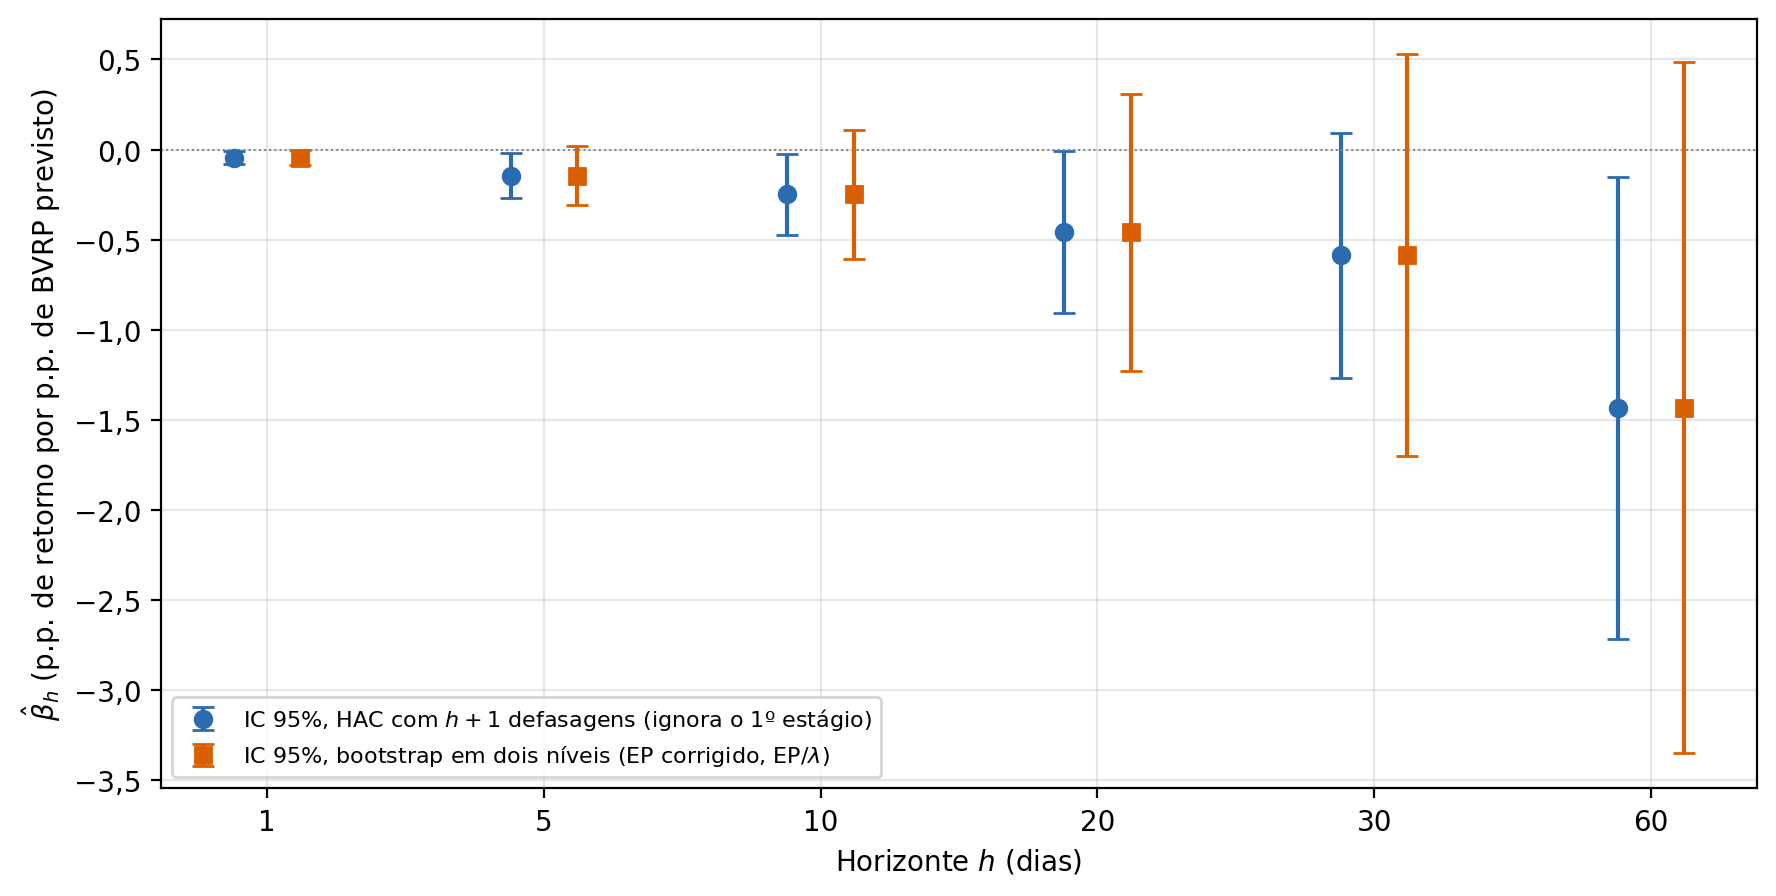
\includegraphics[width=0.9\linewidth]{figs/retornos_linear/fig_betas.png}
    \caption{Coeficiente do retorno futuro sobre o BVRP previsto (Ridge), por horizonte, com intervalos de confiança de 95\%: erro-padrão HAC com $h+1$ defasagens, que ignora a estimação do BVRP previsto, e bootstrap em dois níveis com o erro-padrão corrigido da atenuação.}
    \label{fig:retlin-betas}
\end{figure}
}{}

Como os seis horizontes são fortemente correlacionados --- os $\beta^*$ de
horizontes vizinhos têm correlação de 0,8 a 0,97 ---, a dissertação testa
também a hipótese conjunta de $\beta_h = 0$ em todos eles
(Tabela~\ref{tab:retlin-conjunto}). O teste de Wald com a covariância dos
$\beta^*$ não rejeita ($p = 0{,}37$), e o resultado se mantém com blocos de 30
e 90 dias ($p = 0{,}21$ e $0{,}27$). O max-$|t|$, um teste de passo único que
toma o maior $|z_h|$ entre os horizontes e tira o valor crítico da
distribuição do máximo nas reamostragens \citep{westfall1993resampling}, em
aplicação com bootstrap em dados dependentes como a de
\citet{romano2005stepwise}, também não rejeita: o menor valor-$p$ ajustado é
0,115, em $h = 1$. A hipótese conjunta só é rejeitada quando a estimação do
BVRP previsto é ignorada: com o HAC das seis regressões empilhadas
($p = 0{,}019$) e com o bootstrap só do segundo nível, que mantém as previsões
fixas ($p = 0{,}032$). A diferença entre os dois grupos de testes é o efeito
do regressor gerado.

\begin{table}[H]
\centering
\small
\caption{Teste conjunto nos seis horizontes.}
\label{tab:retlin-conjunto}
\begin{tabular}{lrrr}
\toprule
Inferência & $W$ & $p$ (Wald) & $p$ (max-$|t|$) \\
\midrule
Dois níveis, blocos de 60 dias (principal) & 6{,}46 & 0{,}373 & 0{,}115 \\
Dois níveis, blocos de 30 dias & 8{,}45 & 0{,}207 & 0{,}135 \\
Dois níveis, blocos de 90 dias & 7{,}59 & 0{,}269 & 0{,}149 \\
Dois níveis, $\alpha$ reescolhido & 4{,}08 & 0{,}666 & 0{,}173 \\
Só o 2º nível (ignora o 1º estágio) & 13{,}76 & 0{,}032 & 0{,}022 \\
HAC empilhado, 61 defasagens (ignora o 1º estágio) & 15{,}11 & 0{,}019 & -- \\
\midrule
\multicolumn{4}{l}{\textit{max-$|t|$ por horizonte (principal), valor-$p$ ajustado}} \\
\multicolumn{4}{l}{$h = 1$: 0{,}115; $h = 5$: 0{,}193; $h = 10$: 0{,}345; $h = 20$: 0{,}485; $h = 30$: 0{,}578; $h = 60$: 0{,}290} \\
\bottomrule
\end{tabular}
\par\smallskip
\parbox{0.95\linewidth}{\footnotesize\textit{Nota}: $H_0$: $\beta_h = 0$ nos seis horizontes. Wald: $W = \bar\beta^{*\prime}\,\Sigma^{*-1}\,\bar\beta^*$, com a média e a covariância dos $\beta^*$ do bootstrap, $\chi^2(6)$; equivale ao teste na escala corrigida da atenuação. max-$|t|$: o maior $|z_h|$ entre os horizontes, com valor crítico tirado da distribuição do máximo nas reamostragens (passo único). HAC empilhado: as seis regressões estimadas em conjunto, com Newey--West. Os $\beta^*$ de horizontes vizinhos têm correlação de 0,8 a 0,97, e o número de condição da matriz de correlação é 475.}
\end{table}


A direção do resultado é a mesma de \citet{bollerslev2009expected}. Com
$\text{BVRP} = \text{VH} - \text{IV}$, um $\beta_h$ negativo equivale a dizer
que um prêmio de variância maior, com a IV acima da volatilidade histórica
futura, antecede retornos maiores. A evidência aqui, porém, é fraca: nenhum
horizonte é significante depois das correções.

% =========================================================
\section{Testes de robustez}
\label{sec:retlin-robustez}

A Tabela~\ref{tab:retlin-robustez} reporta os valores-$p$ do bootstrap em
variantes do procedimento. Com blocos de 30 e de 90 dias, os valores-$p$ ficam
entre 0,042 e 0,42; com o $\alpha$ do Ridge reescolhido em cada reamostragem,
entre 0,068 e 0,57. Com a previsão da floresta aleatória, o coeficiente
também é negativo em todos os horizontes e de magnitude parecida, mas nenhum é
significante (valores-$p$ HAC entre 0,15 e 0,61). Só o bootstrap do segundo
nível, que ignora o primeiro estágio, tem um horizonte abaixo do limite de
Bonferroni ($h = 1$, $p = 0{,}003$). O sinal é estável; a significância não
é.

\begin{table}[H]
\centering
\small
\caption{Testes de robustez: valores-$p$ por horizonte.}
\label{tab:retlin-robustez}
\begin{tabular}{lrrrrrr}
\toprule
Variante & $h = 1$ & $h = 5$ & $h = 10$ & $h = 20$ & $h = 30$ & $h = 60$ \\
\midrule
Blocos de 30 dias & 0{,}042 & 0{,}080 & 0{,}130 & 0{,}167 & 0{,}201 & 0{,}060 \\
Blocos de 90 dias & 0{,}050 & 0{,}098 & 0{,}225 & 0{,}326 & 0{,}423 & 0{,}205 \\
$\alpha$ reescolhido & 0{,}068 & 0{,}156 & 0{,}300 & 0{,}442 & 0{,}573 & 0{,}432 \\
Floresta aleatória & 0{,}498 & 0{,}631 & 0{,}783 & 0{,}808 & 0{,}838 & 0{,}700 \\
Só o 2º nível (ignora o 1º estágio) & 0{,}003 & 0{,}022 & 0{,}058 & 0{,}108 & 0{,}178 & 0{,}080 \\
\addlinespace
Floresta aleatória: $\hat\beta_h$ & $-$0{,}057 & $-$0{,}113 & $-$0{,}142 & $-$0{,}294 & $-$0{,}357 & $-$1{,}235 \\
Floresta aleatória: $p$ HAC & 0{,}148 & 0{,}342 & 0{,}487 & 0{,}493 & 0{,}606 & 0{,}333 \\
\bottomrule
\end{tabular}
\par\smallskip
\parbox{0.95\linewidth}{\footnotesize\textit{Nota}: Valores-$p$ do bootstrap em dois níveis na escala corrigida da atenuação (999 reamostragens; 199 na floresta). Principal: Ridge com o $\alpha$ de cada origem fixo e blocos de 60 dias (Tabela~\ref{tab:retlin-principal}). $\alpha$ reescolhido: validação cruzada refeita em cada treino reamostrado. Só o 2º nível: previsões originais fixas, sem correção. Floresta: $\hat\beta_h$ em p.p. por p.p.}
\end{table}


% =========================================================
\section{Volatilidade histórica e implícita separadas}
\label{sec:retlin-componentes}

A equação~\eqref{eq:met-retorno-componentes} substitui o prêmio por seus
componentes observados em $t$, a volatilidade histórica dos 30 dias anteriores
e a IV. Se $\beta_{1,h} + \beta_{2,h} = 0$, a diferença
$\text{VH}_{t-29:t} - \text{IV}_t$, que é a $\text{BVRP}^{\text{proxy}}_t$,
resume o conteúdo das duas medidas. A Tabela~\ref{tab:retlin-componentes}
mostra que os coeficientes têm sinais opostos de $h = 1$ a $h = 20$, a IV com
sinal positivo, e que a restrição só é rejeitada em $h = 1$ ($p = 0{,}039$;
nos demais horizontes, $p \ge 0{,}18$). Nenhum coeficiente individual é
significante depois da correção de Bonferroni. O teste usa a volatilidade
histórica retrospectiva, a da proxy, e não o BVRP previsto: ele diz se a
diferença entre as duas volatilidades observadas em $t$ é uma forma adequada
de combiná-las, não se o prêmio prospectivo prevê o retorno.

\begin{table}[H]
\centering
\small
\caption{Retorno futuro sobre a volatilidade histórica e a implícita.}
\label{tab:retlin-componentes}
\begin{tabular}{rrrrrrr}
\toprule
$h$ & $\hat\beta_{1,h}$ (VH) & $p$ & $\hat\beta_{2,h}$ (IV) & $p$ & $\hat\beta_{1,h} + \hat\beta_{2,h}$ & $p$ \\
\midrule
1 & $-$0{,}009 & 0{,}233 & 0{,}026 & 0{,}023 & 0{,}017 & 0{,}039 \\
5 & $-$0{,}019 & 0{,}493 & 0{,}061 & 0{,}155 & 0{,}042 & 0{,}183 \\
10 & $-$0{,}031 & 0{,}599 & 0{,}090 & 0{,}329 & 0{,}059 & 0{,}329 \\
20 & $-$0{,}025 & 0{,}832 & 0{,}103 & 0{,}564 & 0{,}078 & 0{,}524 \\
30 & 0{,}005 & 0{,}979 & 0{,}074 & 0{,}776 & 0{,}079 & 0{,}667 \\
60 & 0{,}178 & 0{,}514 & 0{,}046 & 0{,}927 & 0{,}224 & 0{,}551 \\
\bottomrule
\end{tabular}
\par\smallskip
\parbox{0.95\linewidth}{\footnotesize\textit{Nota}: $R_{t+h} = \alpha_h + \beta_{1,h}\,\text{VH}_{t-29:t} + \beta_{2,h}\,\text{IV}_t + \varepsilon_{t+h}$, nas mesmas 987 datas; coeficientes em p.p. de retorno por p.p. de volatilidade. Valores-$p$ HAC com $h+1$ defasagens; a última coluna testa $\beta_{1,h} + \beta_{2,h} = 0$.}
\end{table}


% =========================================================
\section{Regime de volatilidade}
\label{sec:retlin-regime}

A equação~\eqref{eq:met-retorno-regime} permite inclinações diferentes nos
regimes de baixa e de alta volatilidade (Seção~\ref{sec:met-regimes}). Com o
corte fixo, a inclinação é mais negativa no regime de baixa, que reúne 31\%
das datas fora da amostra ($-2{,}92$ em $h = 30$, $p = 0{,}005$), e fica perto
de zero no regime de alta ($-0{,}34$) (Tabela~\ref{tab:retlin-regime}). A
inclinação no regime de baixa passa pelo limite de Bonferroni de $h = 20$ a
$h = 60$, mas a diferença entre os regimes, não: a interação é significante a
5\% de $h = 10$ a $h = 60$, sem passar pelo limite, e o teste conjunto da
variável de regime e da interação só rejeita a 5\% em $h = 60$
($p = 0{,}035$). Com o corte reestimado em cada origem, a diferença deixa de
ser significante (interação com $p \ge 0{,}06$; teste conjunto com
$p \ge 0{,}16$). A diferença entre os regimes é, assim, sugestiva e frágil:
depende da posição do corte, e esses valores-$p$ são do HAC, que ignora a
estimação do BVRP previsto.

\begin{table}[H]
\centering
\small
\caption{Retorno futuro, BVRP previsto e regime de volatilidade.}
\label{tab:retlin-regime}
\begin{tabular}{rrrrrrr}
\toprule
$h$ & Baixa: $\hat\beta_h$ & $p$ & Alta & $\hat\gamma_h$ & $p$ & $p$ (Wald) \\
\midrule
\multicolumn{7}{l}{\textit{Corte fixo} (31{,}4\% das datas no regime de baixa)} \\
1 & $-$0{,}071 & 0{,}155 & $-$0{,}061 & 0{,}011 & 0{,}857 & 0{,}554 \\
5 & $-$0{,}528 & 0{,}034 & $-$0{,}131 & 0{,}396 & 0{,}140 & 0{,}250 \\
10 & $-$1{,}091 & 0{,}015 & $-$0{,}159 & 0{,}932 & 0{,}046 & 0{,}128 \\
20 & $-$2{,}147 & 0{,}006 & $-$0{,}313 & 1{,}834 & 0{,}034 & 0{,}081 \\
30 & $-$2{,}922 & 0{,}005 & $-$0{,}339 & 2{,}583 & 0{,}031 & 0{,}071 \\
60 & $-$5{,}172 & $<$0{,}001 & $-$1{,}034 & 4{,}138 & 0{,}026 & 0{,}035 \\
\addlinespace
\multicolumn{7}{l}{\textit{Corte expansivo} (25{,}1\% das datas no regime de baixa)} \\
1 & $-$0{,}072 & 0{,}227 & $-$0{,}058 & 0{,}014 & 0{,}833 & 0{,}491 \\
5 & $-$0{,}295 & 0{,}176 & $-$0{,}139 & 0{,}156 & 0{,}510 & 0{,}751 \\
10 & $-$0{,}546 & 0{,}145 & $-$0{,}196 & 0{,}350 & 0{,}392 & 0{,}694 \\
20 & $-$1{,}313 & 0{,}055 & $-$0{,}342 & 0{,}971 & 0{,}184 & 0{,}414 \\
30 & $-$2{,}030 & 0{,}037 & $-$0{,}319 & 1{,}711 & 0{,}100 & 0{,}250 \\
60 & $-$4{,}397 & 0{,}005 & $-$1{,}077 & 3{,}319 & 0{,}064 & 0{,}159 \\
\bottomrule
\end{tabular}
\par\smallskip
\parbox{0.95\linewidth}{\footnotesize\textit{Nota}: $R_{t+h} = \alpha_h + \beta_h\,\widehat{\text{BVRP}}_t + \delta_h D_t + \gamma_h D_t\,\widehat{\text{BVRP}}_t + \varepsilon_{t+h}$, com $D_t = 1$ no regime de alta volatilidade. Inclinação no regime de baixa: $\hat\beta_h$; no de alta: $\hat\beta_h + \hat\gamma_h$; em p.p. por p.p. Valores-$p$ HAC com $h+1$ defasagens; Wald: $\delta_h = \gamma_h = 0$. Corte fixo: $37{,}3\%$ a.a., da primeira janela; expansivo: reestimado em cada origem.}
\end{table}


% =========================================================
\section{Síntese}
\label{sec:retlin-sintese}

O BVRP previsto tem relação negativa e estável com os retornos futuros em
todos os horizontes, na direção prevista pela literatura, mas a relação não é
significante quando a inferência considera a estimação do BVRP previsto e as
comparações múltiplas. O modelo linear não prevê os retornos do Bitcoin nesta
amostra. Os horizontes longos têm pouco poder, e a ausência de significância
neles não é evidência de ausência de relação. A diferença entre os regimes de
volatilidade, sugestiva com o corte fixo, motiva o
Capítulo~\ref{chap:retornos_nao_linear}, em que um modelo em árvore escolhe
sozinho os cortes.
